\chapter{Diseño e implementación de los modelos o técnicas necesarias}\label{ch: modelDesign}
En el capítulo \ref{ch: eda} se expuso la naturaleza espectral del problema, sería lógico pensar que una forma de reducir el ruido de una conversación sería filtrar para todas aquellas frecuencias que no sean la frecuencia fundamental y sus armónicos característicos del habla de una persona. Esta solución sería perfectamente válida y se ajusta a la necesidad del problema pero tiene un gran inconveniente, el tuneo fino y adaptable de los filtros.

Para poder filtrar las frecuencias fundamentales, éstas deben ser encontradas y esa no es tarea fácil. Además dichas frecuencias varían en el tiempo de modo que los filtros deben adaptarse a cada instante a la nuevas frecuencias, esto complica la tarea aún más. Existe una familia de filtros llamados \textit{comb}, peine, que consisten en una serie de picos equi-espaciados creando mediante retardos de la propia señal perfectamente válidos para la detección y filtrado de la frecuencia fundamental\cite{1035730}, de nuevo el tuneo fino es una tarea compleja. Por ello, este trabajo propone un sistema completo de redes neuronales en el cual no se aplican técnicas de clásicas de \gls{DSP}.

Dado que el en capítulo \ref{ch: eda} se presentaron los análisis en frecuencia y en tiempo, quedó de manifiesto que en el dominio de la frecuencia las pistas con ruido y sin él se diferencian mucho. Por esta razón el algoritmo que se propone en este trabajo se basa en el análisis de audio en el dominio de la frecuencia, para ello se deben pre-procesar los datos eligiendo unos parámetros que determinarán como serán los datos, a continuación se explican los algoritmos matemáticos de las transformaciones que se van a aplicar a las pistas de audio.

\section{Preprocesado de datos de audio para el modelo}
Los modelos se van a alimentar de \glspl{FFT} calculadas a partir de las muestras temporales de los audios. Estas \glspl{FFT} deben ser lo suficientemente precisas para poder reconstruir el audio pero sin usar una gran cantidad de muestras para no producir un retraso en la señal.

Se ha realizado una prueba experimental para calcular a que tasa de muestreo el audio sigue siendo posible reconstruir. A menor tasa de muestreo, para la misma resolución en frecuencia, la \gls{FFT} resultante tiene menos puntos, i.e., menor carga computacional. Es importante este ajuste porque reducir la tasa de muestreo a la mitad o un cuarto implica reducir el vector de entrada de la red a la mitad o un cuarto, respectivamente. Adicionalmente sólo son procesados la mitad de los datos de la salida de la transformada de Fourier. Esto es debido a que la respuesta de una transformada es un vector de números complejos y de éstos sólo se procesa el módulo. La fase se deja intacta y se usa para reconstruir el vector complejo junto con el módulo que sale del modelo. La figura \ref{fig: model_schema} presenta un esquema de cuáles son las entradas y salidas del modelo.

\begin{figure}[ht!]
	\centering
	\resizebox{\textwidth}{!}{
		\begin{tikzpicture}
		\tikzstyle{box} = [draw,inner sep=7,minimum size=57,line 
		width=1, very thick, draw=black, fill=black!20, text width=100, text centered]
		\tikzstyle{invisible} = [outer sep=0,inner sep=0,minimum size=0]
		\tikzstyle{stealth} = [-stealth, very thick]
		\begin{scope}[shift={(0.5,0)}]		
		\begin{scope}[shift={(-3.5,3.1)}, scale=0.5]
		\node [invisible] at (-1.2,1.7) {$FFT_n$};
		\draw (-3,0.5) node [invisible] {} -- (-2.8,0.3) node [invisible] {} -- (-2.6,0.2) node [invisible] {} -- (-2.4,0.8) node [invisible] {} -- (-2.2,0.2) node [invisible] {} -- (-2,0.3) node [invisible] {} -- (-1.9,0.2) node [invisible] {} -- (-1.8,0.4) node [invisible] {} -- (-1.7,0.2) node [invisible] {} -- (-1.6,1.4) node [invisible] {} -- (-1.5,0.2) node [invisible] {} -- (-1.3,0.3) node [invisible] (v4) {};
		\node [invisible] (v2) at (-3,1.6) {};
		\node [invisible] (v1) at (-3,-0.4) {};
		\node [invisible] (v3) at (0.6,-0.4) {};
		\draw [stealth] (v1) edge (v2);
		\draw [stealth] (v1) edge (v3);
		\draw [stealth](v4);
		\draw (v4) -- (-1.2,0.2) node [invisible] {} -- (-1.1,0.4) node [invisible] {} -- (-1,0.2) node [invisible] {} -- (-0.8,0.8) node [invisible] {} -- (-0.7,0.2) node [invisible] {} -- (-0.5,0.3) node [invisible] {} -- (-0.4,0.2) node [invisible] {} -- (-0.2,0.3) node [invisible] {} -- (-0.1,0.2) node [invisible] {} -- (0.1,1.1) node [invisible] {} -- (0.3,0.2) node [invisible] {};
		\end{scope}
		\begin{scope}[shift={(-3.1,1.8)}, scale=0.5]
		\node [invisible] at (-1.2,1.7) {$FFT_{n-1}$};
		\draw (-3,0.5) node [invisible] {} -- (-2.8,0.3) node [invisible] {} -- (-2.6,0.2) node [invisible] {} -- (-2.4,0.8) node [invisible] {} -- (-2.2,0.2) node [invisible] {} -- (-2,0.3) node [invisible] {} -- (-1.9,0.2) node [invisible] {} -- (-1.8,0.4) node [invisible] {} -- (-1.7,0.2) node [invisible] {} -- (-1.6,1.4) node [invisible] {} -- (-1.5,0.2) node [invisible] {} -- (-1.3,0.3) node [invisible] (v4) {};
		\node [invisible] (v2) at (-3,1.6) {};
		\node [invisible] (v1) at (-3,-0.4) {};
		\node [invisible] (v3) at (0.6,-0.4) {};
		\draw [stealth] (v1) edge (v2);
		\draw [stealth] (v1) edge (v3);
		\draw [stealth](v4);
		\draw (v4) -- (-1.2,0.2) node [invisible] {} -- (-1.1,0.4) node [invisible] {} -- (-1,0.2) node [invisible] {} -- (-0.8,0.8) node [invisible] {} -- (-0.7,0.2) node [invisible] {} -- (-0.5,0.3) node [invisible] {} -- (-0.4,0.2) node [invisible] {} -- (-0.2,0.3) node [invisible] {} -- (-0.1,0.2) node [invisible] {} -- (0.1,1.1) node [invisible] {} -- (0.3,0.2) node [invisible] {};
		\end{scope}
		\begin{scope}[shift={(-1.5,-0.9)}, scale=0.5]
		\node [invisible] at (-1.2,1.7) {$FFT_2$};
		\draw (-3,0.5) node [invisible] {} -- (-2.8,0.3) node [invisible] {} -- (-2.6,0.2) node [invisible] {} -- (-2.4,0.8) node [invisible] {} -- (-2.2,0.2) node [invisible] {} -- (-2,0.3) node [invisible] {} -- (-1.9,0.2) node [invisible] {} -- (-1.8,0.4) node [invisible] {} -- (-1.7,0.2) node [invisible] {} -- (-1.6,1.4) node [invisible] {} -- (-1.5,0.2) node [invisible] {} -- (-1.3,0.3) node [invisible] (v4) {};
		\node [invisible] (v2) at (-3,1.6) {};
		\node [invisible] (v1) at (-3,-0.4) {};
		\node [invisible] (v3) at (0.6,-0.4) {};
		\draw [stealth] (v1) edge (v2);
		\draw [stealth] (v1) edge (v3);
		\draw [stealth](v4);
		\draw (v4) -- (-1.2,0.2) node [invisible] {} -- (-1.1,0.4) node [invisible] {} -- (-1,0.2) node [invisible] {} -- (-0.8,0.8) node [invisible] {} -- (-0.7,0.2) node [invisible] {} -- (-0.5,0.3) node [invisible] {} -- (-0.4,0.2) node [invisible] {} -- (-0.2,0.3) node [invisible] {} -- (-0.1,0.2) node [invisible] {} -- (0.1,1.1) node [invisible] {} -- (0.3,0.2) node [invisible] {};
		\end{scope}
		\begin{scope}[shift={(-1.1,-2.2)}, scale=0.5]
		\node [invisible] at (-1.2,1.7) {$FFT_1$};
		\draw (-3,0.5) node [invisible] {} -- (-2.8,0.3) node [invisible] {} -- (-2.6,0.2) node [invisible] {} -- (-2.4,0.8) node [invisible] {} -- (-2.2,0.2) node [invisible] {} -- (-2,0.3) node [invisible] {} -- (-1.9,0.2) node [invisible] {} -- (-1.8,0.4) node [invisible] {} -- (-1.7,0.2) node [invisible] {} -- (-1.6,1.4) node [invisible] {} -- (-1.5,0.2) node [invisible] {} -- (-1.3,0.3) node [invisible] (v4) {};
		\node [invisible] (v2) at (-3,1.6) {};
		\node [invisible] (v1) at (-3,-0.4) {};
		\node [invisible] (v3) at (0.6,-0.4) {};
		\draw [stealth] (v1) edge (v2);
		\draw [stealth] (v1) edge (v3);
		\draw [stealth](v4);
		\draw (v4) -- (-1.2,0.2) node [invisible] {} -- (-1.1,0.4) node [invisible] {} -- (-1,0.2) node [invisible] {} -- (-0.8,0.8) node [invisible] {} -- (-0.7,0.2) node [invisible] {} -- (-0.5,0.3) node [invisible] {} -- (-0.4,0.2) node [invisible] {} -- (-0.2,0.3) node [invisible] {} -- (-0.1,0.2) node [invisible] {} -- (0.1,1.1) node [invisible] {} -- (0.3,0.2) node [invisible] {};
		\end{scope}
		\node [circle, fill] at (-3.6,1.2) {};
		\node [circle, fill] at (-3.2,0.8) {};
		\node [circle, fill] at (-2.8,0.4) {};
		\draw [dashed, thick] (-5.5,6) node [invisible] (v5) {} -- (-5.5,-3.5) -- (-0.5,-3.5) -- (-0.5,6) -- (v5);
		\node [invisible] (v6) at (-0.5,0.75) {};
		\end{scope}
		
		\begin{scope}[shift={(10.5,0)}]		
		\begin{scope}[shift={(-1.2,3.1)}, scale=0.5]
		\node [invisible] at (-1.2,1.7) {$FFT_n$};
		\draw (-3,0.5) node [invisible] {} -- (-2.8,0.3) node [invisible] {} -- (-2.6,0.2) node [invisible] {} -- (-2.4,0.8) node [invisible] {} -- (-2.2,0.2) node [invisible] {} -- (-2,0.3) node [invisible] {} -- (-1.9,0.2) node [invisible] {} -- (-1.8,0.4) node [invisible] {} -- (-1.7,0.2) node [invisible] {} -- (-1.6,1.4) node [invisible] {} -- (-1.5,0.2) node [invisible] {} -- (-1.3,0.3) node [invisible] (v4) {};
		\node [invisible] (v2) at (-3,1.6) {};
		\node [invisible] (v1) at (-3,-0.4) {};
		\node [invisible] (v3) at (0.6,-0.4) {};
		\draw [stealth] (v1) edge (v2);
		\draw [stealth] (v1) edge (v3);
		\draw [stealth](v4);
		\draw (v4) -- (-1.2,0.2) node [invisible] {} -- (-1.1,0.4) node [invisible] {} -- (-1,0.2) node [invisible] {} -- (-0.8,0.8) node [invisible] {} -- (-0.7,0.2) node [invisible] {} -- (-0.5,0.3) node [invisible] {} -- (-0.4,0.2) node [invisible] {} -- (-0.2,0.3) node [invisible] {} -- (-0.1,0.2) node [invisible] {} -- (0.1,1.1) node [invisible] {} -- (0.3,0.2) node [invisible] {};
		\end{scope}
		\begin{scope}[shift={(-1.7,1.8)}, scale=0.5]
		\node [invisible] at (-1.2,1.7) {$FFT_{n-1}$};
		\draw (-3,0.5) node [invisible] {} -- (-2.8,0.3) node [invisible] {} -- (-2.6,0.2) node [invisible] {} -- (-2.4,0.8) node [invisible] {} -- (-2.2,0.2) node [invisible] {} -- (-2,0.3) node [invisible] {} -- (-1.9,0.2) node [invisible] {} -- (-1.8,0.4) node [invisible] {} -- (-1.7,0.2) node [invisible] {} -- (-1.6,1.4) node [invisible] {} -- (-1.5,0.2) node [invisible] {} -- (-1.3,0.3) node [invisible] (v4) {};
		\node [invisible] (v2) at (-3,1.6) {};
		\node [invisible] (v1) at (-3,-0.4) {};
		\node [invisible] (v3) at (0.6,-0.4) {};
		\draw [stealth] (v1) edge (v2);
		\draw [stealth] (v1) edge (v3);
		\draw [stealth](v4);
		\draw (v4) -- (-1.2,0.2) node [invisible] {} -- (-1.1,0.4) node [invisible] {} -- (-1,0.2) node [invisible] {} -- (-0.8,0.8) node [invisible] {} -- (-0.7,0.2) node [invisible] {} -- (-0.5,0.3) node [invisible] {} -- (-0.4,0.2) node [invisible] {} -- (-0.2,0.3) node [invisible] {} -- (-0.1,0.2) node [invisible] {} -- (0.1,1.1) node [invisible] {} -- (0.3,0.2) node [invisible] {};
		\end{scope}
		\begin{scope}[shift={(-3.2,-0.9)}, scale=0.5]
		\node [invisible] at (-1.2,1.7) {$FFT_2$};
		\draw (-3,0.5) node [invisible] {} -- (-2.8,0.3) node [invisible] {} -- (-2.6,0.2) node [invisible] {} -- (-2.4,0.8) node [invisible] {} -- (-2.2,0.2) node [invisible] {} -- (-2,0.3) node [invisible] {} -- (-1.9,0.2) node [invisible] {} -- (-1.8,0.4) node [invisible] {} -- (-1.7,0.2) node [invisible] {} -- (-1.6,1.4) node [invisible] {} -- (-1.5,0.2) node [invisible] {} -- (-1.3,0.3) node [invisible] (v4) {};
		\node [invisible] (v2) at (-3,1.6) {};
		\node [invisible] (v1) at (-3,-0.4) {};
		\node [invisible] (v3) at (0.6,-0.4) {};
		\draw [stealth] (v1) edge (v2);
		\draw [stealth] (v1) edge (v3);
		\draw [stealth](v4);
		\draw (v4) -- (-1.2,0.2) node [invisible] {} -- (-1.1,0.4) node [invisible] {} -- (-1,0.2) node [invisible] {} -- (-0.8,0.8) node [invisible] {} -- (-0.7,0.2) node [invisible] {} -- (-0.5,0.3) node [invisible] {} -- (-0.4,0.2) node [invisible] {} -- (-0.2,0.3) node [invisible] {} -- (-0.1,0.2) node [invisible] {} -- (0.1,1.1) node [invisible] {} -- (0.3,0.2) node [invisible] {};
		\end{scope}
		\begin{scope}[shift={(-3.7,-2.2)}, scale=0.5]
		\node [invisible] at (-1.2,1.7) {$FFT_1$};
		\draw (-3,0.5) node [invisible] {} -- (-2.8,0.3) node [invisible] {} -- (-2.6,0.2) node [invisible] {} -- (-2.4,0.8) node [invisible] {} -- (-2.2,0.2) node [invisible] {} -- (-2,0.3) node [invisible] {} -- (-1.9,0.2) node [invisible] {} -- (-1.8,0.4) node [invisible] {} -- (-1.7,0.2) node [invisible] {} -- (-1.6,1.4) node [invisible] {} -- (-1.5,0.2) node [invisible] {} -- (-1.3,0.3) node [invisible] (v4) {};
		\node [invisible] (v2) at (-3,1.6) {};
		\node [invisible] (v1) at (-3,-0.4) {};
		\node [invisible] (v3) at (0.6,-0.4) {};
		\draw [stealth] (v1) edge (v2);
		\draw [stealth] (v1) edge (v3);
		\draw [stealth](v4);
		\draw (v4) -- (-1.2,0.2) node [invisible] {} -- (-1.1,0.4) node [invisible] {} -- (-1,0.2) node [invisible] {} -- (-0.8,0.8) node [invisible] {} -- (-0.7,0.2) node [invisible] {} -- (-0.5,0.3) node [invisible] {} -- (-0.4,0.2) node [invisible] {} -- (-0.2,0.3) node [invisible] {} -- (-0.1,0.2) node [invisible] {} -- (0.1,1.1) node [invisible] {} -- (0.3,0.2) node [invisible] {};
		\end{scope}
		\node [circle, fill] at (-2.8,1.2) {};
		\node [circle, fill] at (-3.2,0.8) {};
		\node [circle, fill] at (-3.6,0.4) {};
		\draw [dashed, thick] (-5.5,6) node [invisible] (v5) {} -- (-5.5,-3.5) -- (-0.5,-3.5) -- (-0.5,6) -- (v5);
		\node [invisible] (v8) at (-5.5,0.75) {};
		\end{scope}
		
		\node [box,text width=60] (v7) at (2.5,0.75) {Modelo};
		
		
		\node [invisible] at (-2.5,5.5) {Módulo de FFT con ruido};
		\node [invisible] at (7.5,5.5) {Módulo de FFT sin ruido};
		\draw [stealth] (v6) edge (v7);
		\draw [stealth] (v7) edge (v8);
		\node [box] (v9) at (-8.5,7) {$Tiempo\xrightarrow{FFT}Frecuencia$};
		\node [box] (v10) at (13.5,7) {$Frecuencia\xrightarrow{iFFT}Tiempo$};
		\node [invisible] (v11) at (-5,0.75) {};
		\node [invisible] (v12) at (10,0.75) {};
		\draw [stealth,out=0,in=180] (v9) edge node[anchor=south]{Fase} (v10);
		\draw [stealth,out=0,in=180] (v9) edge node[anchor=east]{Módulo}(v11);
		\draw [stealth,out=0,in=180] (v12) edge node[anchor=west]{Módulo}(v10);
		\end{tikzpicture}
	}      
	\caption{Esquema de las entradas y salidas de datos del modelo}
	\label{fig: model_schema}
\end{figure}


\subsection{Generación de datos de entrenamiento y validación}

\section{Modelo de capas \acrshort{LSTM}}

\subsection{Tipos de arquitectura}

